\chapter{Lighting Controller}
The first element of the system to be developed was the lighting controller.
This part of the project had no prior development, so all contributions were done from scratch.

The lighting controller has a simple function in this system; it maps processed biosignals to lighting position and intensity.
Therefore, it should be able to communicate with the off-body PC and pass various commands through to the lights connected to it.

During the planning stage of the project, DMX was determined to be the most appropriate protocol to use for this purpose.
Additionally, both a off-the-shelf controller, and prototyping fixture are to be developed to give the project robustness,
while allowing for cost-effective prototyping.


\section{Methods}
Off-the-shelf controllers were researched and an appropriate controller was chosen.
The only device that was within the project's budget while providing an open source driver, for aid in development,
was the ENTEC OpenDMX controller.

While the controller was being ordered, a prototyping fixture was developed.
The choice of parts used for this fixture came from what was available as to not add additional cost to the project.
The fixture was made using an Arduino and eight NeoPixel LEDs.

The Arduino was programmed such that the eight NeoPixels could be controlled via DMX frames.
The DMX frame is sent via serial over USB
and the Arduino maps intensity, red, green, and blue channels for each individual LED, making a total of four channels per LED.

On the off-body PC, the driver for the ENTEC OpenDMX controller is written in C\#.
A C\# program was written to allow control of the device from other languages.
Additionally, Arduino serial communication was integrated to allow the prototyping fixture to be controlled from the same interface.


\section{Results}
The off-the-shelf controller and custom software allows lighting fixtures to be controlled from other high-level languages in real-time,
shown in~\autoref{image:prof_fixture}.
The implementation of this also allows it to be running on a separate PC connected to the network,
if lighting control needed to be done away from the main processing, or to free up resources on the main processing PC.

The off-the-shelf controller has a delay of 25 ms.
It is capable of driving 512 DMX addresses of any kind.

\begin{figure}[h]
\caption{Professional lighting fixture control using off-the-shelf controller and custom driver interface}\label{image:prof_fixture}
\centering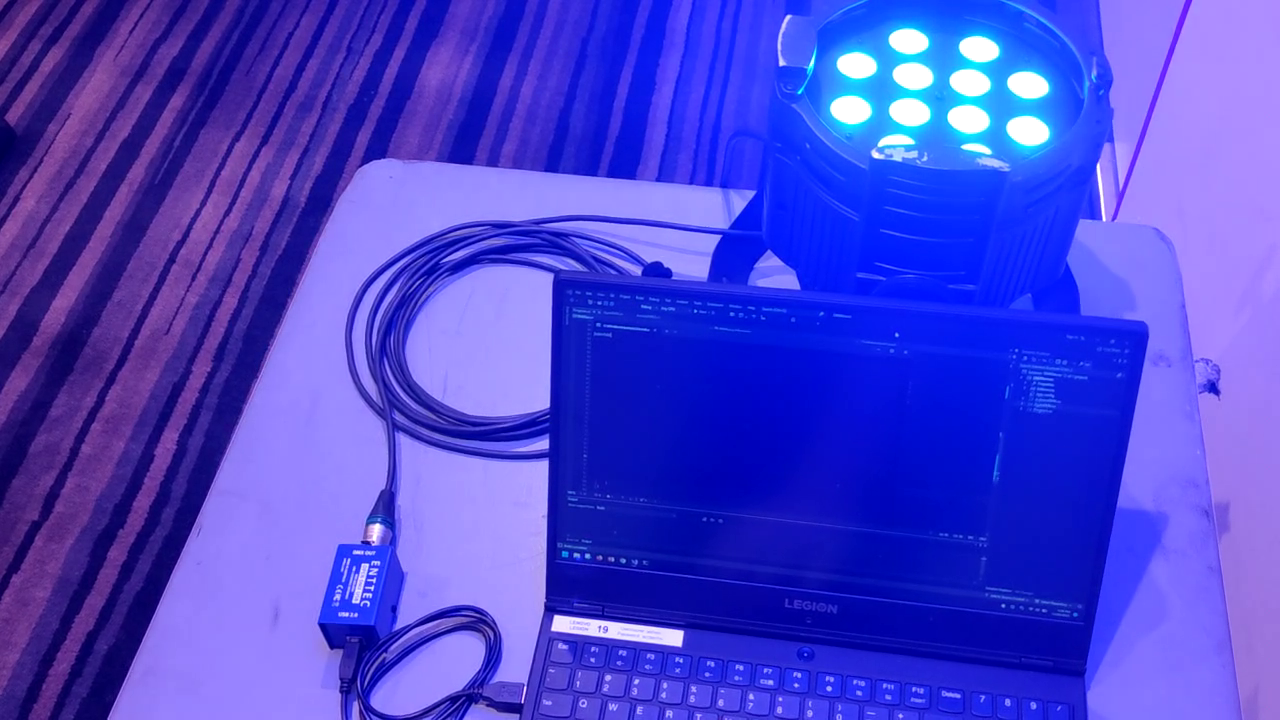
\includegraphics[width=\textwidth]{chapters/development/off_the_shelf_controller}
\end{figure}

The prototyping fixture uses the exact same interface, allowing it to be interchanged with the off-the-shelf controller,
seen in~\autoref{image:proto_fixture}.
Each LED can be controlled independently with red, green, blue, and intensity channels,
making it suitable for simulating larger strings of fixtures.

The prototyping fixture communication has an average delay of 5.56 ms.
It has a total of 32 address that can be individually controlled.
The device has been run for over two hours with no address misalignment.

\begin{figure}[h]
\caption{Prototyping fixture using the same driver interface}\label{image:proto_fixture}
\centering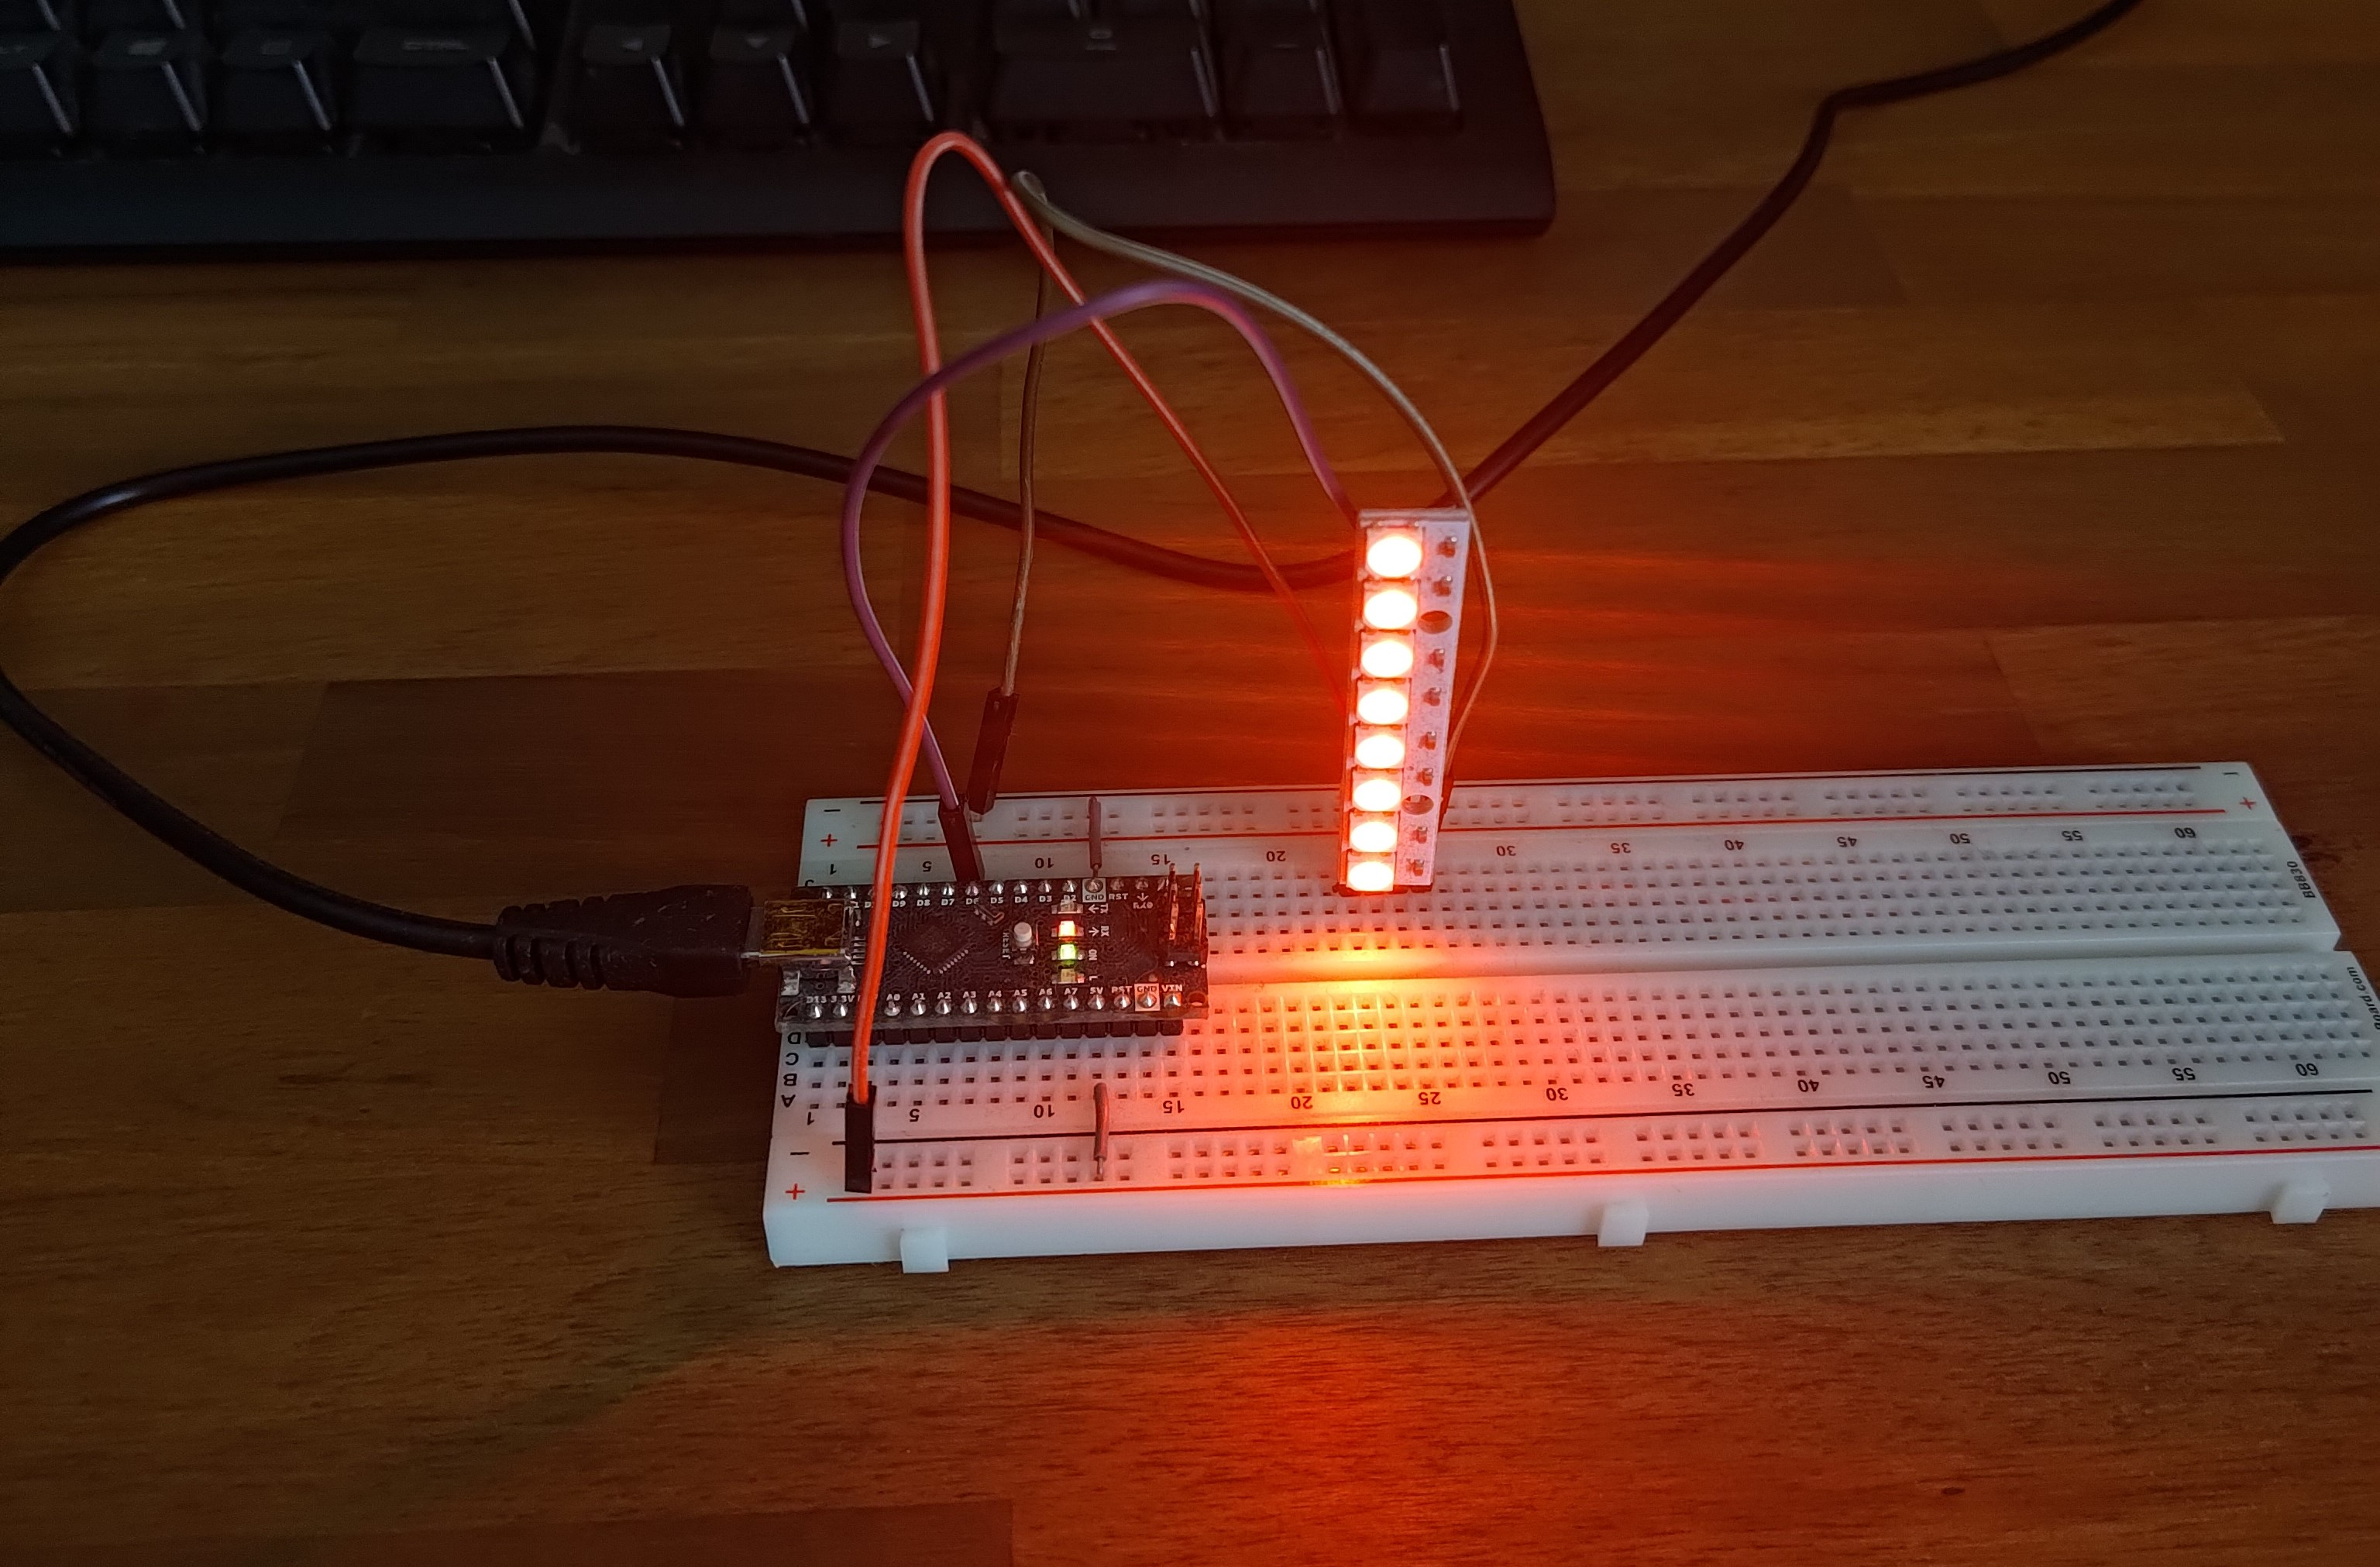
\includegraphics[width=\textwidth]{chapters/development/prototyping_fixture_cropped}
\end{figure}


\section{Discussion}
The implementation of lighting control in this manner allows for rapid development of processing algorithms for multiple lights,
without needing expensive hardware.
This allows performers to fine tune their lighting displays prior the show when they may not have access to the lighting fixtures yet.

Because of the implementation, algorithms that work on the prototyping fixture will also work on the off-the-shelf controller.
The only change necessarily is to update the DMX addresses to match the corresponding fixture address.

The biggest challenge with the implementation of the lighting controller was the prototyping fixture.
DMX is a protocol that sends `frames' of 512 bytes continuously.
Each byte corresponds to a DMX address, the address number is the byte's offset in the 512 byte array.
So, the 12\textsuperscript{th} byte will correspond to the 12\textsuperscript{th} address
and the value of that byte will be what is applied to the fixture at that address.
Frames are sent out multiple times per second, regardless of if any values in the 512 byte array have changed,
so that the fixtures can determine when the controller is unplugged.
For the prototyping fixture receiving DMX over serial, there is no simple way to know where the start of the frame is.
If it is assumed to be when the device first receives serial data,
it may be misaligned due to differences in when the PC starts sending serial DMX frames and when the device first powers on.
Additionally, if data is lost over the transmission, the data will be misaligned with no way of recovering without a reset.

One method to solve this would be to wait for a pause greater than a specific length between characters
and use that to mark the beginning of a new transmission.
However, if different timings were to be used the code would have to be updated and slight delays in transmission could lead to misaligned.

Another method is to mark the end of transmission with a special character.
However, there is no way to distinguish between data and special characters without using an alternative character set.
This is because a byte worth of data constitutes all binary values between `00000000' and `11111111'.
So there would be no way to determine if binary `01000011' was supposed to be interpreted as the character `C' or the number 67.
There are a number of different character sets, for this portion of the project base64~\cite{Sumartono:2016} was chosen.
This is because it only contains printable characters, making each string easier to debug, and it is well documented.
As this is for a prototyping fixture, it is more important to have it be functional than to be as well optimised as something going into production.

The base64 encoded string represents the entire DMX frame.
To reduce unnecessary processing, the frame is reduced to only 32 addresses, which is the number of addresses used by the fixture.
Before the frame is base64 encoded, each address concatenated into a single string that represents the entire DMX frame.
To make the addresses easier to separate, as well as to ensure both the base64 string and the decoded string are a fixed length,
the addresses are sent as a fixed three-digit decimal number.
These three-digit numbers are concatenated into a string and base64 encoded before being sent to the Arduino.
This makes debugging easier, as the numbers can be directly read as their decimal representation before they are encoded and once they are decoded.
Extracting the numbers is simpler because each number has a known position and can be simply converted from a string into a number,
and storing the strings is easier as they are constant lengths, so fixed length buffers can be used,
which is favourable on a limited memory device like an Arduino.
